\chapter{Desarrollo}

\section{Descripción general}

Para describir el desarrollo se ha decidido seguir el estándar IEEE 830 para la especificación de requisitos \footnote{\url{www.fdi.ucm.es/profesor/Gmendez/docs/is0809/ieee830.pdf}}.

\section{Perspectiva del producto}

El sistema a construir consistirá en una aplicación móvil para dispositivos Android \footnote{\url{www.android.com}} desarrollada con el motor de videojuegos Unity3D \footnote{\url{https://unity3d.com/es/}}. 

La aplicación no formará parte de un sistema mayor, será un videojuego totalmente independiente. Aun así se hará uso de servicios de terceros tales como librerías de software, frameworks y APIs entre otros.

\section{Funcionalidad del producto}

Resumen de las funcionalidades principales que el producto debe realizar, sin entrar en información de detalle.
El videojuego deberá permitir el movimiento del jugador en el plano 2D, además podrá interactuar con los NPCs y dialogar con ellos. Se podrán completar objetivos y logros para de este modo avanzar en la historia.

El juego además enseñará conceptos clave sobre \textquote{Lean Startup} y sobre el emprendimiento en general.

\section{Características de los usuarios}

El perfil de un consumidor de formación sobre emprendimiento es muy amplio: desde jóvenes recién graduados llenos de optimismo hasta personas de mediana edad que desean reinventarse y dejar de ser asalariados. 

Es por ello que es difícil concretar un perfil ya que son diferentes personas de diferentes edades y perfiles socioculturales las que desean aventurarse en el emprendimiento.

En cualquier caso sí se pueden encontrar aspectos comunes en esta gran variaded de usuarios:

\begin{itemize}

\item conocimiento tecnológico y como desenvolverse con aplicaciones móviles
\item interés por el mundo del emprendimiento y la empresa
\item interés por los videojuegos
\item interés por los videojuegos educativos

\end{itemize}

\section{Restricciones}

Existen varias limitaciones a tener en cuenta a la hora de diseñar y desarrollar el sistema:

\begin{itemize}

\item para la realización del proyecto se dispondrá de un presupuesto nulo. Es por ello que las herramientas, frameworks y demás productos que se utilicen deberán ser gratuitas.
\item el motor de videojuegos a utilizar deberá ser Unity 3D ya que se tiene conocimiento del mismo y no se dispone de tiempo para aprender a utilizar otro motor de videojuegos.
\item el lenguaje de programación a utilizar será C\# ya que de entre los disponibles para Unity 3D es el más adecuado por potencia, documentación y dominio por parte del desarrollador.
\item el sistema operativo objetivo será Android ya junto con los sistemas operativos para ordenador no requiere ninguna licencia para publicar aplicaciones. La plataforma serán los dispositivos móviles ya que es muy sencillo llegar al público de esta plataforma, aunque no tanto hacerse hueco entre dicha audiencia.

\end{itemize}

\section{Requisitos específicos}

\subsection{Interfaces de usuario}

Respecto a las interfaces de usuario se pueden observar dos estilos claramente diferenciados: las interfaces del menú principal y las de la pantalla de juego. En cuanto a las primeras deberán seguir un estilo minimalista y utilizar controles simples; respecto de las segundas, la simplicidad es obligatoria.

Es un requisito imprescindible que la interfaz mostrada durante el juego no sea intrusiva y entorpezca la experiencia de usuario. Esto se conseguirá disponiendo pequeños botones en la pantalla situados de forma estratégica para que la visión del jugador se centre principalmente en el mundo del juego y los personajes.

Un requisito común de las interfaces de usuario es que debido a que serán mostradas en un dispositivo móvil tendrán que adecuarse a una pantalla pequeña y recibir la interacción del usuario mediante toques en la pantalla del dispositivo.

\subsection{Requisitos funcionales}

Para describir las funcionalidades del sistema se utilizará una aproximación basada en mecánicas. Cada posible acción del usuario sobre el sistema se considerará una mecánica y se definirá como un requisito. 

Dichas mecánicas son activadas al detectarse cierto estímulo. Por ejemplo al producir el estímulo de tocar en algun lugar del mundo, se desencadena la mecánica de movimiento.

Al identificador de cada funcionalidad le acompañarán unas siglas (USR, UI, SYS) dependiendo de si dicha funcionalidad se refiere a mecánicas del usuario, la interfaz de usuario o al sistema.

\subsection{Requisitos de usuario}
\label{requisitosUsuario}

\begin{table}[H]
\centering
\label{my-label}
\begin{tabular}{|l|l|}
\hline
\textbf{Identificador} & RF-USR-01                                                                                                                                                              \\ \hline
\textbf{Nombre}        & Mover personaje                                                                                                                                                        \\ \hline
\textbf{Requerimiento} & El usuario podrá elegir donde mover al personaje controlado                                                                                                            \\ \hline
\textbf{Descripción}   & \begin{tabular}[c]{@{}l@{}}Al tocar con el dedo en cualquier punto de la pantalla el personaje\\   controlado se moverá a esa posición (solo en el eje x)\end{tabular} \\ \hline
\textbf{Prioridad}     & Imprescindible                                                                                                                                                         \\ \hline
\end{tabular}
\end{table}

\begin{table}[H]
\centering
\label{my-label}
\begin{tabular}{|l|l|}
\hline
\textbf{Identificador} & RF-USR-02                                                                                                                                           \\ \hline
\textbf{Nombre}        & Interactuar con NPCs                                                                                                                                \\ \hline
\textbf{Requerimiento} & El usuario podrá seleccionar un NPC con el que interactuar                                                                                          \\ \hline
\textbf{Descripción}   & \begin{tabular}[c]{@{}l@{}}Al tocar con el dedo sobre un NPC, si se está lo suficientemente cerca se\\   abrirá el menú conversacional\end{tabular} \\ \hline
\textbf{Prioridad}     & Imprescindible                                                                                                                                      \\ \hline
\end{tabular}
\end{table}

\begin{table}[H]
\centering
\label{my-label}
\begin{tabular}{|l|l|}
\hline
\textbf{Identificador} & RF-USR-03                                                                                                                                      \\ \hline
\textbf{Nombre}        & Cambiar de escenario                                                                                                                           \\ \hline
\textbf{Requerimiento} & Se podrá navegar entre escenarios                                                                                                              \\ \hline
\textbf{Descripción}   & \begin{tabular}[c]{@{}l@{}}Al clicar en una de las puertas de cada escenario se avanzará al\\   escenario asociado a dicha puerta\end{tabular} \\ \hline
\textbf{Prioridad}     & Imprescindible                                                                                                                                 \\ \hline
\end{tabular}
\end{table}

\subsection{Requisitos de interfaz}

\begin{table}[H]
\centering
\label{my-label}
\begin{tabular}{|l|l|}
\hline
\textbf{Identificador} & RF-UI-01                                                                                                                                                \\ \hline
\textbf{Nombre}        & Navegar menú principal                                                                                                                                  \\ \hline
\textbf{Requerimiento} & Se podrá cambiar entre las diferentes pantallas del menú principal                                                                                      \\ \hline
\textbf{Descripción}   & \begin{tabular}[c]{@{}l@{}}Arrastrando con el dedo en la pantalla hacia la derecha/izquierda se\\   cambiará a la correspondiente pantalla\end{tabular} \\ \hline
\textbf{Prioridad}     & Imprescindible                                                                                                                                          \\ \hline
\end{tabular}
\end{table}

\begin{table}[H]
\centering
\label{my-label}
\begin{tabular}{|l|l|}
\hline
\textbf{Identificador} & RF-UI-02                                                                                                                                        \\ \hline
\textbf{Nombre}        & Comenzar juego                                                                                                                                  \\ \hline
\textbf{Requerimiento} & \begin{tabular}[c]{@{}l@{}}Se empezará el juego al seleccionar el botón correspondiente en el menú\\   principal\end{tabular}                   \\ \hline
\textbf{Descripción}   & \begin{tabular}[c]{@{}l@{}}En el el menú principal en la vista inicial se podrá comenzar el juego al\\   presionar el botón "play"\end{tabular} \\ \hline
\textbf{Prioridad}     & Imprescindible                                                                                                                                  \\ \hline
\end{tabular}
\end{table}

\begin{table}[H]
\centering
\label{my-label}
\begin{tabular}{|l|l|}
\hline
\textbf{Identificador} & RF-UI-03                                                                                                                            \\ \hline
\textbf{Nombre}        & Desactivar/Activar música                                                                                                           \\ \hline
\textbf{Requerimiento} & Se podrá desactivar la música ambiente del juego                                                                                    \\ \hline
\textbf{Descripción}   & \begin{tabular}[c]{@{}l@{}}Clicando en el icono de Música en el menú de opciones se\\   activará/desactivará la música\end{tabular} \\ \hline
\textbf{Prioridad}     & Baja                                                                                                                                \\ \hline
\end{tabular}
\end{table}

\begin{table}[H]
\centering
\label{my-label}
\begin{tabular}{|l|l|}
\hline
\textbf{Identificador} & RF-UI-04                                                                                                                                           \\ \hline
\textbf{Nombre}        & Desactivar/Activar sonidos                                                                                                                         \\ \hline
\textbf{Requerimiento} & Se podrán desactivar los efectos de sonido del juego                                                                                               \\ \hline
\textbf{Descripción}   & \begin{tabular}[c]{@{}l@{}}Clicando en el icono de Sonidos en el menú de opciones se\\   activarán/desactivarán los efectos de sonido\end{tabular} \\ \hline
\textbf{Prioridad}     & Baja                                                                                                                                               \\ \hline
\end{tabular}
\end{table}

\begin{table}[H]
\centering
\label{my-label}
\begin{tabular}{|l|l|}
\hline
\textbf{Identificador} & RF-UI-05                                                                                                                                          \\ \hline
\textbf{Nombre}        & Eliminar logros                                                                                                                                   \\ \hline
\textbf{Requerimiento} & Se podrán eliminar los logros conseguidos                                                                                                         \\ \hline
\textbf{Descripción}   & \begin{tabular}[c]{@{}l@{}}Clicando en el icono de Eliminar logros del menú de opciones se\\   eliminarán todos los logros obtenidos\end{tabular} \\ \hline
\textbf{Prioridad}     & Baja                                                                                                                                              \\ \hline
\end{tabular}
\end{table}

\begin{table}[H]
\centering
\label{my-label}
\begin{tabular}{|l|l|}
\hline
\textbf{Identificador} & RF-UI-06                                                                                                                                                              \\ \hline
\textbf{Nombre}        & Ver otros juegos                                                                                                                                                      \\ \hline
\textbf{Requerimiento} & Se podrá acceder a la descarga de otros juegos del autor                                                                                                              \\ \hline
\textbf{Descripción}   & \begin{tabular}[c]{@{}l@{}}Clicando en los iconos de juegos del apartado "Mas juegos" se\\   accederá a Google Play donde se podrá descargar dicho juego\end{tabular} \\ \hline
\textbf{Prioridad}     & Baja                                                                                                                                                                  \\ \hline
\end{tabular}
\end{table}

\begin{table}[H]
\centering
\label{my-label}
\begin{tabular}{|l|l|}
\hline
\textbf{Identificador} & RF-UI-07                                                                                                                                                                           \\ \hline
\textbf{Nombre}        & Navegar entre logros                                                                                                                                                               \\ \hline
\textbf{Requerimiento} & Se podrán seleccionar logros y ver su descripción                                                                                                                                  \\ \hline
\textbf{Descripción}   & \begin{tabular}[c]{@{}l@{}}En el menú de logros se podrá navegar entre los logros usando las flechas\\   de navegación y ver la descripción y la imagen de los mismos\end{tabular} \\ \hline
\textbf{Prioridad}     & Media                                                                                                                                                                              \\ \hline
\end{tabular}
\end{table}

\begin{table}[H]
\centering
\label{my-label}
\begin{tabular}{|l|l|}
\hline
\textbf{Identificador} & RF-UI-08                                                                                                                                                                    \\ \hline
\textbf{Nombre}        & Ver logros desbloquados                                                                                                                                                     \\ \hline
\textbf{Requerimiento} & Se podrá ver la cantidad de logros desbloqueados hasta el momento                                                                                                           \\ \hline
\textbf{Descripción}   & \begin{tabular}[c]{@{}l@{}}En el menú de logros aparecerá un texto representando el número de logros\\   desbloqueados hasta el momento y el total a conseguir\end{tabular} \\ \hline
\textbf{Prioridad}     & Baja                                                                                                                                                                        \\ \hline
\end{tabular}
\end{table}

\begin{table}[H]
\centering
\label{my-label}
\begin{tabular}{|l|l|}
\hline
\textbf{Identificador} & RF-UI-09                                                                                                                  \\ \hline
\textbf{Nombre}        & Ver descripción de logro                                                                                                  \\ \hline
\textbf{Requerimiento} & Se podrá ver una descripción de los logros                                                                                \\ \hline
\textbf{Descripción}   & \begin{tabular}[c]{@{}l@{}}En el menú de logros se podrá ver un texto descriptivo del logro\\   seleccionado\end{tabular} \\ \hline
\textbf{Prioridad}     & Media                                                                                                                     \\ \hline
\end{tabular}
\end{table}

\begin{table}[H]
\centering
\label{my-label}
\begin{tabular}{|l|l|}
\hline
\textbf{Identificador} & RF-UI-10                                                                                                                                                                                                               \\ \hline
\textbf{Nombre}        & Navegar entre logros                                                                                                                                                                                                   \\ \hline
\textbf{Requerimiento} & Se podrá seleccionar el logro del que se desea ver información                                                                                                                                                         \\ \hline
\textbf{Descripción}   & \begin{tabular}[c]{@{}l@{}}En el menú de logros se podrá navegar entre logros tocando y arrastrando\\   en la lista de logros. El logro que se sitúe en el centro de la pantalla será\\   el logro activo\end{tabular} \\ \hline
\textbf{Prioridad}     & Media                                                                                                                                                                                                                  \\ \hline
\end{tabular}
\end{table}

\begin{table}[H]
\centering
\label{my-label}
\begin{tabular}{|l|l|}
\hline
\textbf{Identificador} & RF-UI-11                                                                                                                                                                                                                                         \\ \hline
\textbf{Nombre}        & Abrir selector de personaje                                                                                                                                                                                                                      \\ \hline
\textbf{Requerimiento} & Se podrá abrir un menú donde seleccionar el personaje a controlar                                                                                                                                                                                \\ \hline
\textbf{Descripción}   & \begin{tabular}[c]{@{}l@{}}Clicando en el icono del selector de personaje se abrirá una ventana con\\   los iconos de cada personaje. El icono del personaje actualmente controlado\\   se mostrará en gris y no será seleccionable\end{tabular} \\ \hline
\textbf{Prioridad}     & Imprescindible                                                                                                                                                                                                                                   \\ \hline
\end{tabular}
\end{table}

\begin{table}[H]
\centering
\label{my-label}
\begin{tabular}{|l|l|}
\hline
\textbf{Identificador} & RF-UI-12                                                                                                                                                                                                                 \\ \hline
\textbf{Nombre}        & Seleccionar personaje                                                                                                                                                                                                    \\ \hline
\textbf{Requerimiento} & Al clicar en un icono de personaje se cambiará el personaje seleccionado                                                                                                                                                 \\ \hline
\textbf{Descripción}   & \begin{tabular}[c]{@{}l@{}}Al clicar en uno de los iconos de personaje se cambia el personaje\\   controlado. En el icono del selector de personaje aparecerá el icono del\\   nuevo personaje seleccionado\end{tabular} \\ \hline
\textbf{Prioridad}     & Imprescindible                                                                                                                                                                                                           \\ \hline
\end{tabular}
\end{table}

\begin{table}[H]
\centering
\label{my-label}
\begin{tabular}{|l|l|}
\hline
\textbf{Identificador} & RF-UI-13                                                              \\ \hline
\textbf{Nombre}        & Cerrar selector de personaje                                          \\ \hline
\textbf{Requerimiento} & Se podrá cerrar el menú donde seleccionar el personaje a controlar    \\ \hline
\textbf{Descripción}   & Clicando en el selector de personaje, si este está abierto se cerrará \\ \hline
\textbf{Prioridad}     & Imprescindible                                                        \\ \hline
\end{tabular}
\end{table}

\begin{table}[H]
\centering
\label{my-label}
\begin{tabular}{|l|l|}
\hline
\textbf{Identificador} & RF-UI-14                                                                                                                                                                                                                        \\ \hline
\textbf{Nombre}        & Notificar objetivo completado                                                                                                                                                                                                   \\ \hline
\textbf{Requerimiento} & Cuando se cumpla el objetivo actual se mostrará una notificación                                                                                                                                                                \\ \hline
\textbf{Descripción}   & \begin{tabular}[c]{@{}l@{}}Al completar un objetivo el icono del indicador de objetivos girará. El\\   texto del nuevo objetivo se añadirá a la lista de objetivos. El objetivo\\   completado se mostrará tachado\end{tabular} \\ \hline
\textbf{Prioridad}     & Media                                                                                                                                                                                                                           \\ \hline
\end{tabular}
\end{table}

\begin{table}[H]
\centering
\label{my-label}
\begin{tabular}{|l|l|}
\hline
\textbf{Identificador} & RF-UI-15                                                                                                                                                                                    \\ \hline
\textbf{Nombre}        & Abrir indicador de objetivos                                                                                                                                                                \\ \hline
\textbf{Requerimiento} & Se podrá abrir la lista de objetivos                                                                                                                                                        \\ \hline
\textbf{Descripción}   & \begin{tabular}[c]{@{}l@{}}Al clicar en el icono del indicador de objetivos se desplegará una lista\\   con los objetivos completados tachados y el objetivo actual sin tachar\end{tabular} \\ \hline
\textbf{Prioridad}     & Media                                                                                                                                                                                       \\ \hline
\end{tabular}
\end{table}

\begin{table}[H]
\centering
\label{my-label}
\begin{tabular}{|l|l|}
\hline
\textbf{Identificador} & RF-UI-16                                                                                                                                \\ \hline
\textbf{Nombre}        & Cerrar indicador de objetivos                                                                                                           \\ \hline
\textbf{Requerimiento} & Se podrá cerrar la lista de objetivos                                                                                                   \\ \hline
\textbf{Descripción}   & \begin{tabular}[c]{@{}l@{}}Al clicar en el icono del indicador de objetivos se cerrará la lista si\\   esta estaba abierta\end{tabular} \\ \hline
\textbf{Prioridad}     & Media                                                                                                                                   \\ \hline
\end{tabular}
\end{table}

\begin{table}[H]
\centering
\label{my-label}
\begin{tabular}{|l|l|}
\hline
\textbf{Identificador} & RF-UI-17                                                                                                                                                                                                                                       \\ \hline
\textbf{Nombre}        & Abrir menú conversacional                                                                                                                                                                                                                      \\ \hline
\textbf{Requerimiento} & Se abrirá el menú conversacional al interactuar con un personaje                                                                                                                                                                               \\ \hline
\textbf{Descripción}   & \begin{tabular}[c]{@{}l@{}}Al abrir el menú conversacional se hará zoom sobre los personajes\\   involucrados. Se mostrará un texto en la pantalla correspondiente a lo que\\   dice el NPC y botones con las posibles respuestas\end{tabular} \\ \hline
\textbf{Prioridad}     & Imprescindible                                                                                                                                                                                                                                 \\ \hline
\end{tabular}
\end{table}

\begin{table}[H]
\centering
\label{my-label}
\begin{tabular}{|l|l|}
\hline
\textbf{Identificador} & RF-UI-18                                                                                                                         \\ \hline
\textbf{Nombre}        & Contestar NPC                                                                                                                    \\ \hline
\textbf{Requerimiento} & Se podrá contestar a los NPC usando el menú conversacional                                                                       \\ \hline
\textbf{Descripción}   & \begin{tabular}[c]{@{}l@{}}Clicando en uno de los botones se contestará al NPC y se actualizará la\\   conversación\end{tabular} \\ \hline
\textbf{Prioridad}     & Imprescindible                                                                                                                   \\ \hline
\end{tabular}
\end{table}

\begin{table}[H]
\centering
\label{my-label}
\begin{tabular}{|l|l|}
\hline
\textbf{Identificador} & RF-UI-19                                                                                                                                                                                                                                                                                             \\ \hline
\textbf{Nombre}        & Terminar conversación                                                                                                                                                                                                                                                                                \\ \hline
\textbf{Requerimiento} & \begin{tabular}[c]{@{}l@{}}Al alcanzar cierto punto de la conversación se cerrará el menu\\   conversacional\end{tabular}                                                                                                                                                                            \\ \hline
\textbf{Descripción}   & \begin{tabular}[c]{@{}l@{}}Cuando la última decisión tomada tiene asociada tiene la marca\\   correspondiente de fin de conversación el menú conversacional se cerrará. El\\   punto en el que se encuentra la conversación se guarda para retomarla desde\\   ese punto posteriormente\end{tabular} \\ \hline
\textbf{Prioridad}     & Imprescindible                                                                                                                                                                                                                                                                                       \\ \hline
\end{tabular}
\end{table}

\subsection{Requisitos de sistema}

\begin{table}[H]
\centering
\label{my-label}
\begin{tabular}{|l|l|}
\hline
\textbf{Identificador} & RF-SYS-01                                                                                                                                                    \\ \hline
\textbf{Nombre}        & Iniciar menú principal                                                                                                                                       \\ \hline
\textbf{Requerimiento} & \begin{tabular}[c]{@{}l@{}}Al iniciar el juego el menú principal comienza en la vista\\   correspondiente\end{tabular}                                       \\ \hline
\textbf{Descripción}   & \begin{tabular}[c]{@{}l@{}}Al iniciar el juego el menú principal mostrará la vista con el título\\   principal y el botón para iniciar el juego\end{tabular} \\ \hline
\textbf{Prioridad}     & Imprescindible                                                                                                                                               \\ \hline
\end{tabular}
\end{table}

\begin{table}[H]
\centering
\label{my-label}
\begin{tabular}{|l|l|}
\hline
\textbf{Identificador} & RF-SYS-02                                                                                                                                                                                                                                         \\ \hline
\textbf{Nombre}        & Seleccionar personaje                                                                                                                                                                                                                             \\ \hline
\textbf{Requerimiento} & \begin{tabular}[c]{@{}l@{}}Al clicar en un icono del selector de personaje se cambiará el personaje\\   controlado\end{tabular}                                                                                                                   \\ \hline
\textbf{Descripción}   & \begin{tabular}[c]{@{}l@{}}Cuando se clique en un icono del selector de personaje se moverá la\\   cámara hasta enfocar al nuevo personaje seleccionado. Cuando se clique en la\\   pantalla se moverá el nuevo personaje controlado\end{tabular} \\ \hline
\textbf{Prioridad}     & Imprescindible                                                                                                                                                                                                                                    \\ \hline
\end{tabular}
\end{table}

\begin{table}[H]
\centering
\label{my-label}
\begin{tabular}{|l|l|}
\hline
\textbf{Identificador} & RF-SYS-03                                                                                                                                                                                                                                                   \\ \hline
\textbf{Nombre}        & Cargar conversación                                                                                                                                                                                                                                         \\ \hline
\textbf{Requerimiento} & Se cargarán las conversaciones desde archivos de texto                                                                                                                                                                                                      \\ \hline
\textbf{Descripción}   & \begin{tabular}[c]{@{}l@{}}Al abrir el menú conversacional se cargará el fichero de texto\\   correspondiente a la conversación del personaje. Si ya se ha conversado con\\   ese personaje se cargará la conversación desde el punto guardado\end{tabular} \\ \hline
\textbf{Prioridad}     & Imprescindible                                                                                                                                                                                                                                              \\ \hline
\end{tabular}
\end{table}

\begin{table}[H]
\centering
\label{my-label}
\begin{tabular}{|l|l|}
\hline
\textbf{Identificador} & RF-SYS-04                                                                                                                                                                        \\ \hline
\textbf{Nombre}        & Contestar NPC                                                                                                                                                                    \\ \hline
\textbf{Requerimiento} & Al contestar a un NPC se actualizarán las respuestas y el texto del NPC                                                                                                          \\ \hline
\textbf{Descripción}   & \begin{tabular}[c]{@{}l@{}}Al contestar a un NPC se leerá del JSON el nuevo texto y las nuevas\\   respuestas y se actualizará la interfaz para mostrar estos datos\end{tabular} \\ \hline
\textbf{Prioridad}     & Imprescindible                                                                                                                                                                   \\ \hline
\end{tabular}
\end{table}

\begin{table}[H]
\centering
\label{my-label}
\begin{tabular}{|l|l|}
\hline
\textbf{Identificador} & RF-SYS-05                                                                                                                                                                                                                                                                                                                 \\ \hline
\textbf{Nombre}        & Codificar conversaciones                                                                                                                                                                                                                                                                                                  \\ \hline
\textbf{Requerimiento} & \begin{tabular}[c]{@{}l@{}}Las conversaciones estarán codificadas en formato JSON y guardadas en\\   ficheros de texto\end{tabular}                                                                                                                                                                                       \\ \hline
\textbf{Descripción}   & \begin{tabular}[c]{@{}l@{}}Cada NPC tendrá un fichero de texto asociado con la conversación que\\   ofrece en formato JSON. Los elementos del JSON serán nodos con texto y nodos\\   hijos con las respuestas asociadas a ese texto. Las respuestas podrán tener\\   "markups" asociadas que indican eventos\end{tabular} \\ \hline
\textbf{Prioridad}     & Imprescindible                                                                                                                                                                                                                                                                                                            \\ \hline
\end{tabular}
\end{table}

\begin{table}[H]
\centering
\label{my-label}
\begin{tabular}{|l|l|}
\hline
\textbf{Identificador} & RF-SYS-06                                                                                                                                                 \\ \hline
\textbf{Nombre}        & Completar objetivo                                                                                                                                        \\ \hline
\textbf{Requerimiento} & \begin{tabular}[c]{@{}l@{}}Se completarán objetivos al tomar decisiones con la markup\\   correspondiente\end{tabular}                                    \\ \hline
\textbf{Descripción}   & \begin{tabular}[c]{@{}l@{}}Cuando se elige una opción de conversación con la "markup" de\\   objetivo asociada, se completará dicho objetivo\end{tabular} \\ \hline
\textbf{Prioridad}     & Imprescindible                                                                                                                                            \\ \hline
\end{tabular}
\end{table}

\begin{table}[H]
\centering
\label{my-label}
\begin{tabular}{|l|l|}
\hline
\textbf{Identificador} & RF-SYS-07                                                                                                                                                                                                               \\ \hline
\textbf{Nombre}        & Cambiar de escenario                                                                                                                                                                                                    \\ \hline
\textbf{Requerimiento} & Cuando el jugador cambia de escenario se modifica la escena                                                                                                                                                             \\ \hline
\textbf{Descripción}   & \begin{tabular}[c]{@{}l@{}}Cuando se produzca un cambio de escenario se desactivará de la escena el\\   escenario abandonado y el jugador aparecerá en el punto de "spawn"\\   asociado al nuevo escenario\end{tabular} \\ \hline
\textbf{Prioridad}     & Imprescindible                                                                                                                                                                                                          \\ \hline
\end{tabular}
\end{table}

\begin{table}[H]
\centering
\label{my-label}
\begin{tabular}{|l|l|}
\hline
\textbf{Identificador} & RF-SYS-08                                                                                                                                                               \\ \hline
\textbf{Nombre}        & Guardar juego                                                                                                                                                           \\ \hline
\textbf{Requerimiento} & El estado del juego se guardará al salir                                                                                                                                \\ \hline
\textbf{Descripción}   & \begin{tabular}[c]{@{}l@{}}Cuando el usuario salga de la aplicación o al menú principal, el estado\\   del juego se guardará en la memoria del dispositivo\end{tabular} \\ \hline
\textbf{Prioridad}     & Baja                                                                                                                                                                    \\ \hline
\end{tabular}
\end{table}

\begin{table}[H]
\centering
\label{my-label}
\begin{tabular}{|l|l|}
\hline
\textbf{Identificador} & RF-SYS-09                                                                                                                                                                                                                    \\ \hline
\textbf{Nombre}        & Cargar juego                                                                                                                                                                                                                 \\ \hline
\textbf{Requerimiento} & Al iniciar el juego se cargarán las partidas guardadas                                                                                                                                                                       \\ \hline
\textbf{Descripción}   & \begin{tabular}[c]{@{}l@{}}Cuando se inice el juego se cargarán las partidas guardadas en caso de\\   existan. De ser así, al iniciar la partida el mundo se encontrará en el\\   estado de la partida guardada\end{tabular} \\ \hline
\textbf{Prioridad}     & Baja                                                                                                                                                                                                                         \\ \hline
\end{tabular}
\end{table}

\begin{table}[H]
\centering
\label{my-label}
\begin{tabular}{|l|l|}
\hline
\textbf{Identificador} & RF-SYS-10                                                                                                                                                                                                                                                                            \\ \hline
\textbf{Nombre}        & Actualizar conversaciones                                                                                                                                                                                                                                                            \\ \hline
\textbf{Requerimiento} & Al completar un objetivo se actualizan las conversaciones                                                                                                                                                                                                                            \\ \hline
\textbf{Descripción}   & \begin{tabular}[c]{@{}l@{}}Al completar un objetivo en una conversación, todas las demás\\   conversaciones se actualizarán a un punto correspondiente de la misma para\\   reflejar el objetivo completado. Las nuevas conversaciones empezarán desde\\   dicho punto.\end{tabular} \\ \hline
\textbf{Prioridad}     & Imprescindible                                                                                                                                                                                                                                                                       \\ \hline
\end{tabular}
\end{table}

\section{Requisitos no funcionales}

\begin{itemize}

\item Rendimiento: el sistema debe de proporcionar una experiencia de juego óptima. Para ello el flujo de juego debe de ser fluido, sin parones o interrupciones.
\item Usabilidad: el sistema debe de ser sencillo de utilizar. De modo que personas sin un contacto o entrenamiento previo sepan desenvolverse por el sistema
\item Costo: el coste del sistema deberá ser cero

\end{itemize}

\section{Arquitectura del sitema}

Para poder explicar la arquitectura del sistema construido es necesario en primer lugar exponer la arquitectura del motor de videojuegos utilizado. El motivo es que el sistema construido tendrá que cumplir con las normas y reglas del motor, ya que se usarán las herramientas que este provee. Es por ello que se puede afirmar que la arquitectura del videojuego está condicionada y subordinada a la del motor utilizado.

Dado que para la realización de este proyecto se ha utilizado el motor de videojuegos Unity3D \footnote{https://unity3d.com/es/}, se explicará a continuación el diseño de dicho motor.

\subsection{Arquitectura de Unity3D}

Unity3D basa su diseño en el modelo entidad-componente \footnote{https://www.genbetadev.com/programacion-de-videojuegos/diseno-de-videojuegos-orientado-a-entidades-y-componentes}. En este diseño, las entidades del mundo del juego obtienen su funcionalidad mediante la agregación de diferentes componentes. 

En el paradigma de la programación orientada a objetos \footnote{https://desarrolloweb.com/articulos/499.php} el comportamiento de una entidad se define en la clase que la representa. Sin embargo, para reducir la duplicación de código se emplea el mecanismo de la herencia, por el cual una clase puede heredar de otra y de esta forma obtener su comportamiento y ampliarlo. 
El problema que reside en basar el diseño en jerarquías de herencia es que a medida que crece la complejidad del sistema crece el "árbol" que forman las clases. Llegados a este punto es probable que se de el caso en el que se precisa cambiar la funcionalidad de una de las clases, y que al hacerlo se modifique de forma involuntaria el comportamiento de otras clases que heredan de la modificada. Llevando el caso a un punto más extremo, se podría dar la situación en la que el comportamiento de una clase sea incompatible con el comportamiento heredado de una clase padre.

Para solucionar este problema el diseño entidad-componente propone crear entidades que actúen como meros contenedores. Dichos contenedores agregarán componentes que les darán la funcionalidad que los definirá. Por ejemplo tanto un jugador como los objetos del escenario tendrían el componente Mesh (malla gráfica) pero solo el jugador tendría el componente Movement (movimiento). Como se puede observar este diseño es altamente flexible, ya que si se toma la precaución de hacer los componentes lo suficientemente genéricos, se pueden aplicar a varias entidades, de forma que hay una gran reutilización de código. 

Otra ventaja es que se produce un muy bajo acoplamiento ya que las funcionalidades están encapsuladas en los componentes y estos son independientes entre sí.

La forma en la que Unity3D aplica este diseño entidad-componente es mediante el uso de \textquote{Gameobjects} (entidades) y components.
Los \textquote{Gameobjects} son la entidad fundamental en Unity3D: todos los elementos que existan en la escena son un \textquote{Gameobject}. Además todas las entidades en Unity3D (en adelante Gameobjects) incorporan como mínimo un componente. Dicho componente se llama \textquote{Transform} y se encarga de la gestión de la posición, la rotación y la escala del \textquote{Gameobject} que lo posee.

En la siguiente imagen (ver fig. \ref{gameobjectComponents}) se puede observar los componentes que posee el \textquote{Gameobject} Leonardo. 

\begin{figure}[H]
\begin{center}
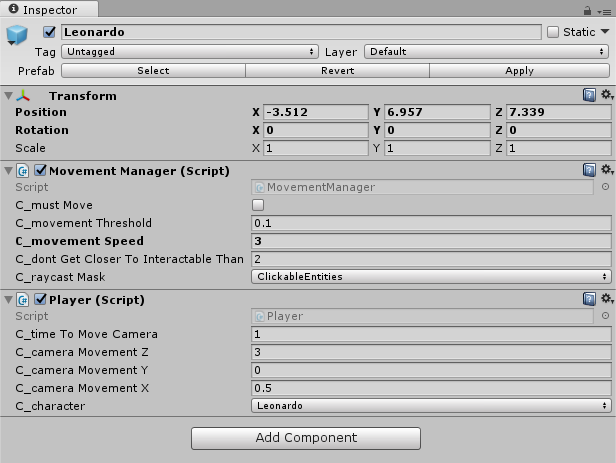
\includegraphics[scale=1]{imagenes/GameobjectsAndComponents.png}
\caption{Vista del editor de Unity3D donde se pueden ver los componentes de un Gameobject}
\label{gameobjectComponents}
\end{center}
\end{figure}

Como se ha mencionado anteriormente el componente \textquote{Transform} es obligatorio en todos \textquote{Gameobjects}. También se pueden ver otros dos componentes, \textquote{Movement Manager} y \textquote{Player}, que han sido creados por el desarrollador.
Dichos componentes dotan a la entidad, que en este caso es el personaje controlable por el jugador, de las características que lo hacen único. Entre otras cosas le dan la habilidad de reaccionar ante los inputs del usuario y moverse por el escenario. También se pueden observar una serie de variables con parámetros. Dado que cada instancia de los componentes es única para la entidad que lo agrega, se pueden personalizar para que incluso entre entidades con los mismos componentes se comporten de manera diferente.

En la siguiente imagen (ver fig. \ref{diagramaClasesUnity}) se puede observar un diagrama de clases que muestra la estructura que compone el sistema de componentes y los Gameobjects.

\begin{figure}[H]
\begin{center}
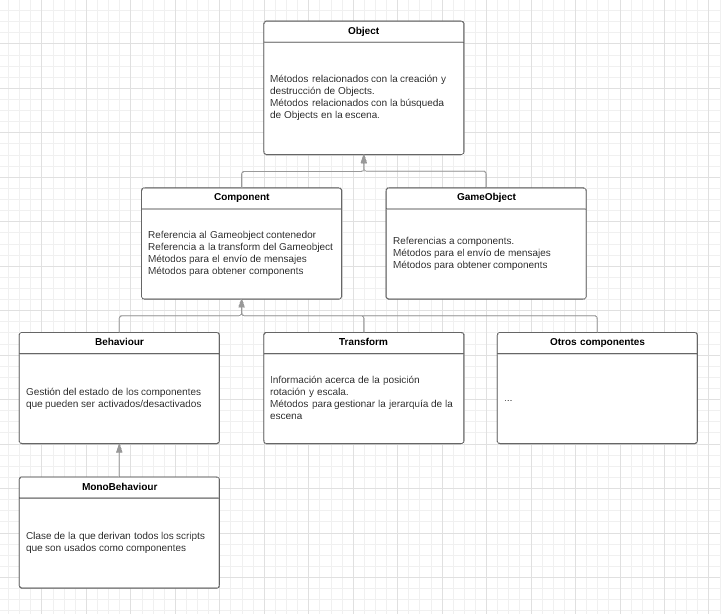
\includegraphics[scale=1]{imagenes/diagramaClasesUnity.png}
\caption{Diagrama de clases de Unity3D}
\label{diagramaClasesUnity}
\end{center}
\end{figure}

Los componentes que provee Unity3D derivan de la clase Component. En el caso de la imagen solo aparece el componente \textquote{Transform}, pero hay muchos más como \textquote{Renderer}, \textquote{Rigidbody}, \textquote{Collider}, etc. En la clase especializada cada componente contendrá la lógica necesaria para desempeñar su función, y el la clase Component se referenciará al \textquote{GameObject} que lo contiene. Cabe notar que un componente no puede existir de forma independiente. Debe estar siempre asociado a una entidad.

La clase MonoBehaviour es también muy importante ya que es la clase base para los scripts creados por los desarrollares. Cualquier fragmento de código que se desee añadir como componente a una entidad deberá heredar de dicha clase. 

Por supuesto se pueden escribir scripts que no hereden de la clase MonoBehaviour, pero en ese caso no podrán ser asignados como componentes a una entidad. Sin embargo no dejan de ser útiles ya que pueden ser usados como POCO \footnote{https://es.wikipedia.org/wiki/Plain\_Old\_CLR\_Object}, definir interfaces, contener lógica o cualquier otra cosa que el desarrollador desee. 

En última instancia los scripts que no heredan de MonoBehaviour deben de ser utilizados desde un script que sí lo haga, ya que este es el único punto de entrada que tienen hacia el sistema de Unity3D.

El último aspecto de la arquitectura que se comentará es el bucle de juego: una parte fundamenta de cualquier videojuego.
El bucle de juego es la parte software más importante en cualquier videojuego. En él se ejecutan las tareas que hacen que el juego 'esté vivo'.
En el siguiente fragmento de código (ver fig. \ref{bucleDeJuego}) se presenta un ejemplo de bucle de juego básico:

\begin{lstlisting}[caption={Código de bucle de juego básico},label=bucleDeJuego]
while(true)
{
	ProcesarInput();
	ActualizarJuego();
	Renderizar();
}
\end{lstlisting}

En este fragmento de código se pueden observar las tres tareas fundamentales de las que se compone cualquier videojuego:

\begin{itemize}
	\item Procesar input: consiste en capturar la interacción del usuario con el sistema mediante el hardware. En esta etapa se puede aplicar algún tipo de filtrado sobre dicho input.
	\item Actualizar juego: se actualiza el estado del juego. Esto consiste en actualizar IA, realizar las acciones del personaje, actualizar el mundo, efectos de objetos, etc.
	\item Renderizar: los elementos del juego se procesan para ser dibujados en la pantalla.
\end{itemize}

El ejemplo de bucle mostrado anteriormente es tremendamente básico pero sirve para explicar las bases de un bucle de juego. Probablemente ningún videojuego moderno lo utilice ya que tiene múltiples inconvenientes como que la frecuencia de actualización del juego dependerá de la carga de trabajo y del rendimiento del sistema que la procese. Actualmente existen variaciones del bucle que solucionan este problema, pero son temas que quedan fuera del alcance de este proyecto.

En la siguiente imagen (ver fig. \ref{bucleUnity}) se puede observar el bucle de juego utilizado por el motor Unity3D, y evidentemente por el juego creado para este proyecto:

\begin{figure}[H]
\begin{center}
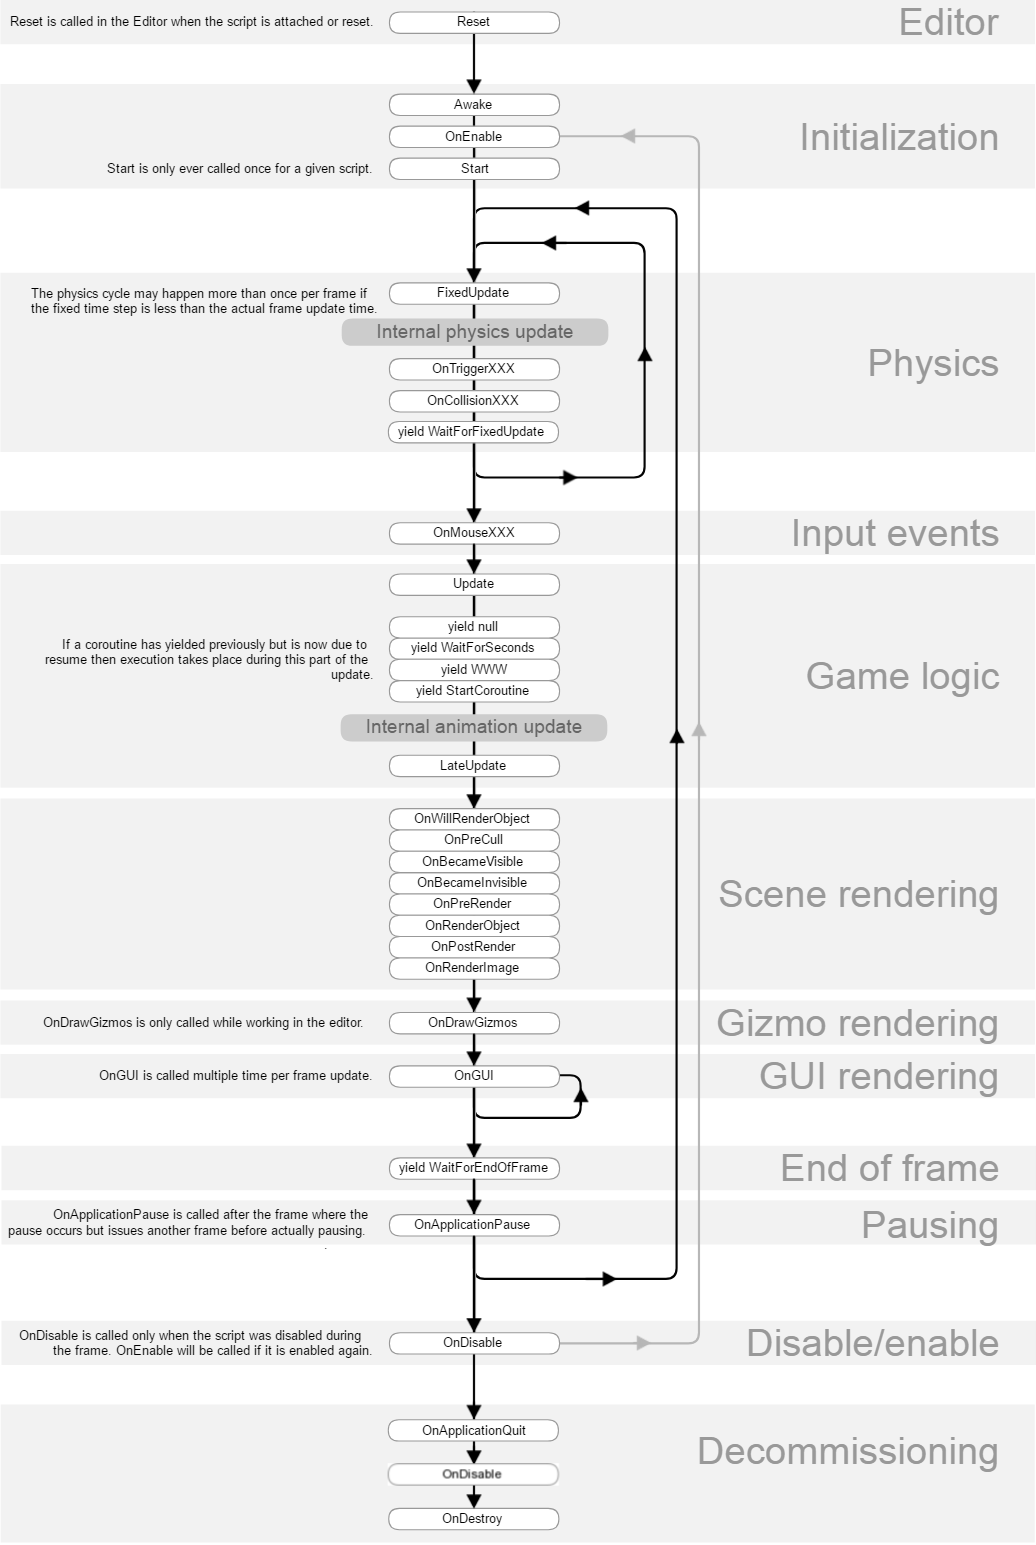
\includegraphics[scale=0.55]{imagenes/bucleUnity.png}
\caption{Bucle de juego del motor Unity3D}
\label{bucleUnity}
\end{center}
\end{figure}

En la imagen se pueden observar las 3 fases clave del bucle de juego: la captura de acciones del jugador, que se produce en la parte denominada como \textquote{Input Events}; la actualización del mundo de juego que se lleva a cabo en \textquote{Physics} y \textquote{Game logic}; finalmente el dibujado del mundo, que se produce en \textquote{Scene rendering}, \textquote{Gizmo rendering} y \textquote{GUI rendering}.


\subsection{Arquitectura del juego}

A continuación se describirá la arquitectura utilizada para desarrollar los componentes más importantes del juego. Estos son: el sistema de conversaciones y el sistema de escenarios. %y el sistema de cambio de personajes , el sistema de movimiento,

\subsubsection{Sistema de conversaciones}

El sistema de conversaciones es el más importante del juego ya que los diálogos con los personajes del juego son el hilo conductor de este.

Los diálogos en lugar de estar insertados directamente en el código se almacenan en ficheros de texto plano independientes. Esto permite que se puedan modificar los diálogos sin tener que recompilar el código del juego. Además permite que cualquier persona sin conocimientos de programación escriba diálogos.

Cada diálogo es un archivo que sigue el formato JSON \footnote{https://geekytheory.com/json-i-que-es-y-para-que-sirve-json}. Las conversaciones tienen una estructura arbórea donde los nodos representan la parte del diálogo correspondiente al NPC y las ramas salientes de dicho nodo representan las posibles contestaciones. La representación de una conversación en el formato JSON sigue la estructura que se puede ver en la siguiente imagen (ver fig. \ref{jsonFormat}).

\begin{figure}[H]
\begin{center}
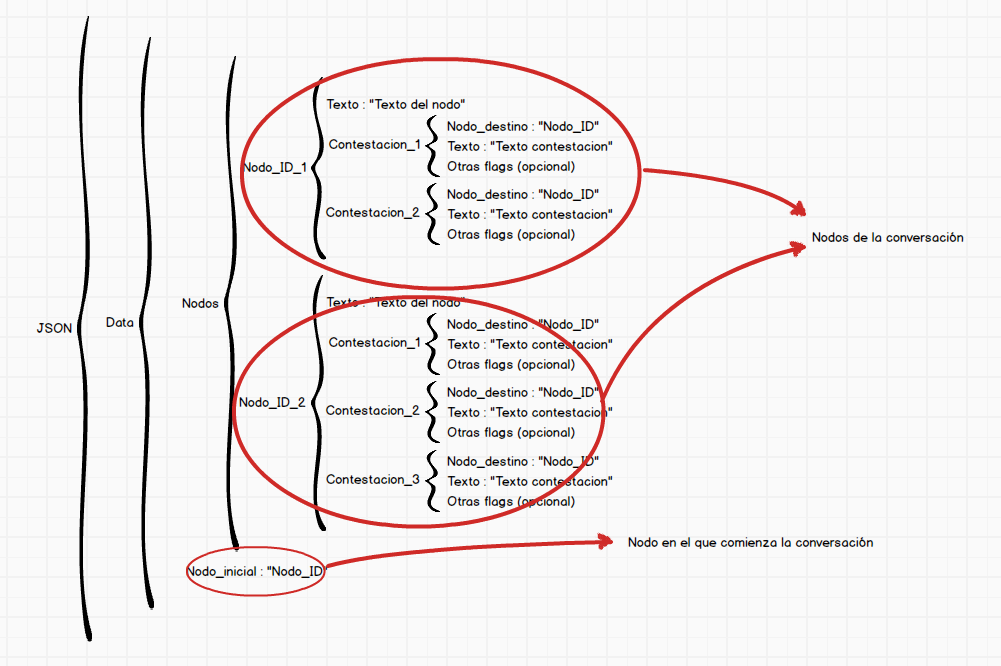
\includegraphics[scale=0.57]{imagenes/jsonFormat.png}
\caption{Representación del formato utilizado para los ficheros de diálogo}
\label{jsonFormat}
\end{center}
\end{figure}

Como se puede observar, los datos contenidos en el JSON son un array de objetos Nodo y un string que indica el nodo inicial de la conversación. 

Los objetos Nodos están indentificados por una cadena de texto que se compone de las tres primeras palabras del diálogo.Cada Nodo contiene el texto del NPC y las posibles contestaciones que el jugador le puede dar.

Las contestaciones se componen de el identificador del nodo al que conduce dicha contestación y el texto de la contestación en sí. Además puede contener ,o no, diferentes \textquote{flags} que le dan a la elección una funcionalidad extra. Entre las \textquote{flags} disponibles se encuentran la de acabar la conversación, desbloquear un objetivo o desbloquear un logro.

Para la creación de los ficheros de diálogos se puede escribir el JSON manualmente rellenando con los datos deseados o se puede utilizar la herramienta inklewritter \footnote{http://www.inklestudios.com/inklewriter/}. Dicha herramienta presenta una forma más sencilla de escribir conversaciones de múltiple respuesta (ver fig. \ref{inklewritter}). Además cuenta con la posibilidad de exportar el trabajo final a un fichero de texto en formato JSON. El parser JSON del videojuego está construido específicamente para poder procesar los diálogos construidos con inklewritter.

\begin{figure}[H]
\begin{center}
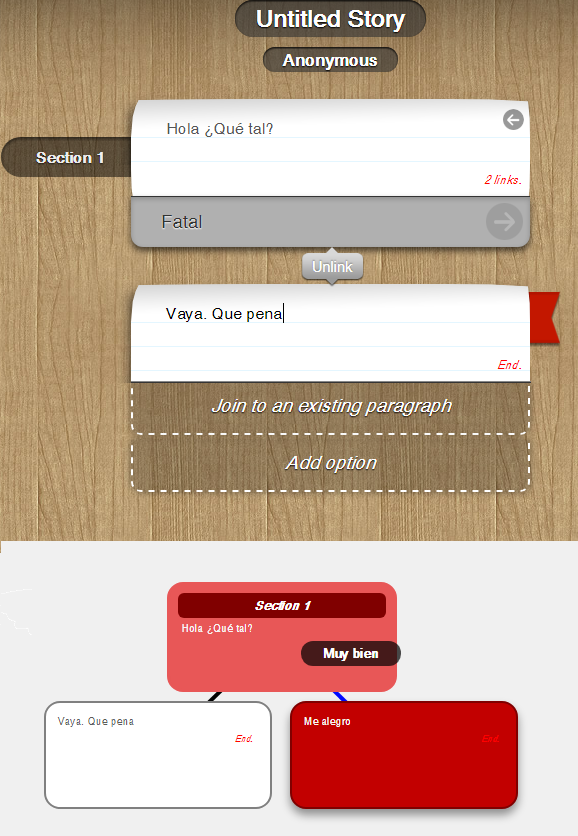
\includegraphics[scale=0.7]{imagenes/inklewritter.png}
\caption{Herramienta inklewritter}
\label{inklewritter}
\end{center}
\end{figure}

Para explicar la arquitectura del sistema de conversaciones se emplearán sendos diagramas de secuencia: uno para explicar el proceso de iniciar una conversación y otro para explicar el proceso de selección de contestaciones.

En el siguiente diagrama (ver fig. \ref{nuevaConversFlujo}) se ve el flujo de código necesario para iniciar una conversación. 

\begin{figure}[H]
\begin{center}
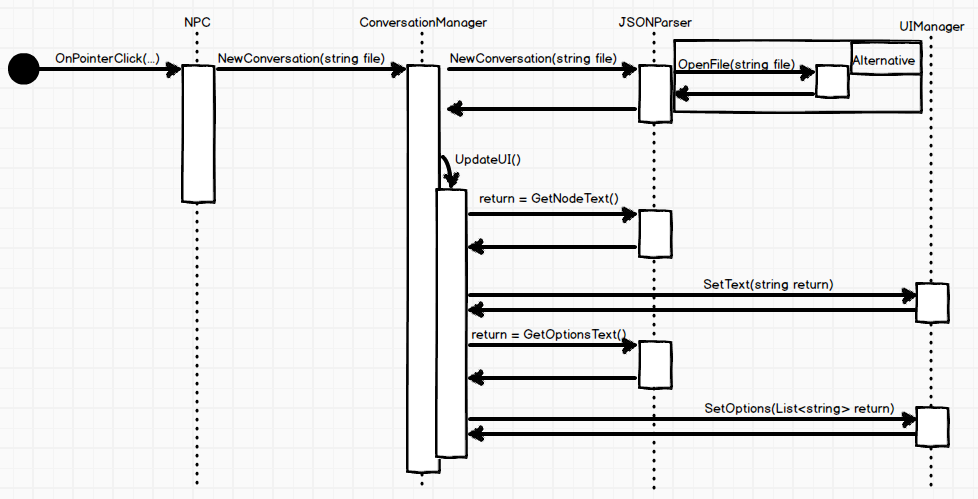
\includegraphics[scale=0.55]{imagenes/nuevaConversFlujo.png}
\caption{Diagrama de flujo nueva conversación}
\label{nuevaConversFlujo}
\end{center}
\end{figure}

No se ha indicado en el diagrama pero para el tratamiento JSON del fichero y para todas las operaciones JSON se utiliza la librería SimpleJSON \footnote{http://wiki.unity3d.com/index.php/SimpleJSON}.


El punto de entrada es el click del jugador en un NPC. Previamente el NPC se habrá registrado en el ConversationManager, de forma que el NPC guarda en un delegado el método NewConversation(string) del ConversationManager.

Cuando se le pide al ConversationManager que inicie una nueva conversación, el NPC le pasa por parámetro la ruta del fichero en la que está almacenado su diálogo con el personaje que está controlando el jugador en ese momento. El ConversationManager informará al JSONParser de que se debe iniciar una nueva conversación, y este será el encargado de leer y parsear el fichero o de abrir una de las conversaciones que tiene almacenadas.

Una vez informado el JSONParser, el ConversationManager le pedirá el texto del nodo actual de la conversación y el texto de las posibles respuestas. Una vez tenga esa información se la pasará al UIManager que se encarga de la interacción con los elementos gráficos de la interfaz.

En este arquitectura se ha seguido un diseño inspirado en el patrón Model-view-Controller \footnote{https://es.wikipedia.org/wiki/Modelo-vista-controlador}. Para ello todas las referencias a los elementos de la interfaz y los métodos de interacción con los mismos se han encapsulado en la clase llama UIManager. El acceso a los datos de las conversaciones, la gestión del estado de las mismas y la lectura de los ficheros de diálogos se guardan en la clase JSONParser, que además utiliza la librería SimpleJSON. En cuanto al punto de encuentro entre los datos y la interfaz, se emplea la clase ConversationManager para sincronizar las operaciones entre las otras dos clases y para proveer un punto de entrada al sistema de conversaciones.

Una vez abierta la conversación es necesario actualizar el juego cada vez que el jugador selecciona una respuesta. El funcionamiento de esta mecánica es muy similar y utiliza los mismos componentes que el sistema anterior.
En el siguiente diagrama de flujo (ver fig. \ref{respuestaFlujo}) se explica el proceso.

\begin{figure}[H]
\begin{center}
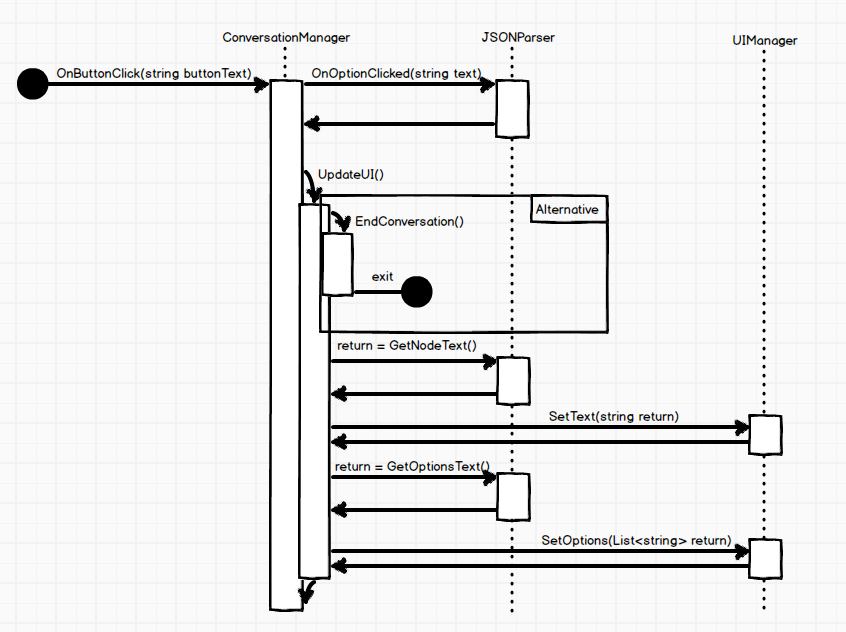
\includegraphics[scale=0.55]{imagenes/respuestaFlujo.png}
\caption{Diagrama de flujo de selección de respuesta}
\label{respuestaFlujo}
\end{center}
\end{figure}

\subsubsection{Sistema de escenarios}

A lo largo del juego se puede navegar por diferentes escenarios. Por temas de eficiencia y debido a que cada escenario tiene características únicas se han agrupado según la temática. En lugar de tener un gran escenario con montones de mallas correspondientes a los edificios y los personajes, solo están activos los Gameobjects correspondientes al escenario actual, los demás están desactivados (que no eliminados). En los escenarios hay puertas que al ser clicadas transportan al personaje activo hacia el escenario al que conduce la puerta. 

En el inspector de escena de Unity3D dichos escenarios lucen como se en la siguiente imagen (ver fig. \ref{unityScenarios}).

\begin{figure}[H]
\begin{center}
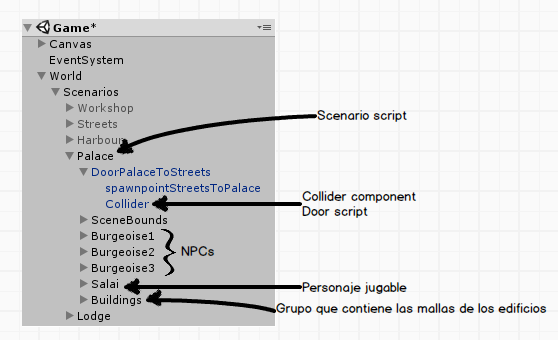
\includegraphics[scale=1]{imagenes/unityScenarios.png}
\caption{Vista de los escenarios en el inspector de Unity3D}
\label{unityScenarios}
\end{center}
\end{figure}

Como se puede observar algunos Gameobjects de la escena contienen scripts y componentes (otros Gameobjects tambien pero se han omitido para mayor simplicidad). En el siguiente diagrama de clases (ver fig. \ref{sceneClassDiagram}) se muestra la estructura de estos scripts y posteriormente se explicará su funcionamiento y utilidad.

\begin{figure}[H]
\begin{center}
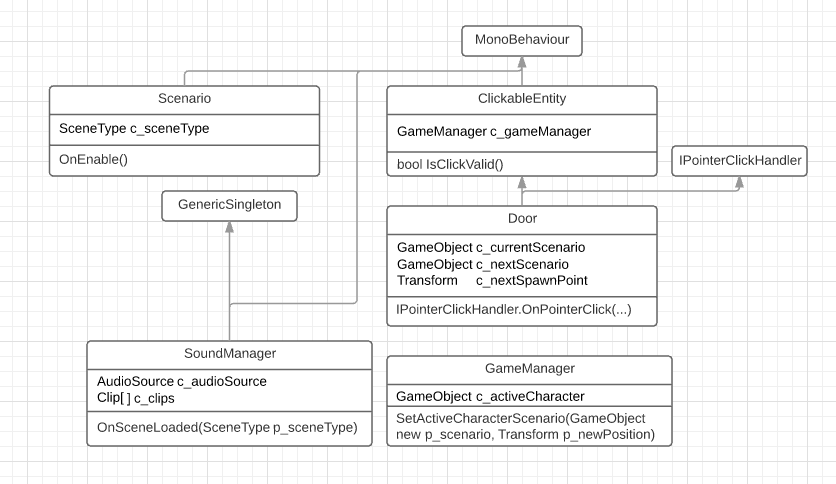
\includegraphics[scale=0.75]{imagenes/sceneClassDiagram.PNG}
\caption{Diagrama de clases del sistema de escenarios}
\label{sceneClassDiagram}
\end{center}
\end{figure}

El elemento central de todo el sistema de escenarios es la puerta. El nombre del Gameobject puerta sigue una notación que indica el escenario destino y origen. En el caso de la imagen anterior (ver fig. \ref{unityScenarios}) se puede observar que la puerta lleva del Palacio (el escenario activo) a Las calles (un escenario desactivado).

El método IPointerClickHandler.OnPointerClick(...), heredado de la interfaz IPointerClickHandler que provee Unity3D, es llamado cuando se hace click en el componente Collider asociado a la puerta. Posteriormente se comprobará que el click es válido (el jugador no está muy lejos por ejemplo) con el método heredado IsClickValid(). Finalmente se notificará al GameManager de que se quiere hacer un cambio de escena y se le suministrará el Gameobject que contiene la nueva escena y la posición de inicio para el jugador.

El sistema de escenarios se encarga también de gestionar la pista de audio que se reproduce a modo de música ambiental. En el objeto raíz de cada escenario se encuentra un script que hace uso del método provisto por Unity3D, OnEnable(). Dicho método es llamado cada vez que se activa un escenario. Desde el método OnEnable() se notifica al SoundManager, que es accesible de forma global ya que implementa el patrón Singleton, el nuevo escenario activado. El SoundManager dispone de un clip de sonido por cada escenario y cuando recibe el tipo del nuevo escenario cambia el clip de sonido reproducido por el componente AudioSource.

\subsection{Storytelling}

El storytelling es una parte fundamental del videojuego creado. Uno de los aspectos que hacen diferente a Da Vinci Startup es que en lugar de saturar al usuario con insufribles lecciones de teoría sobre emprendimiento, se aprende a la vez que se juega. Eso no significa que el conocimiento técnico no esté presente. La diferencia es que el conocimiento se adquiere a lo largo de la historia que los NPCs cuentan y que el jugador experimenta. De este modo conceptos como el "networking" no son solo palabras en un manual, si no que el jugador deberá utilizarlo a lo largo del juego para lograr los objetivos que le llevarán a completar el mismo.


En el \nameref{guionLiterario} contenido en el \nameref{GDD} se explica de forma narrativa la historia en la que se basa el videojuego. Es una historia ficticia en la que un mentor guía a Leonardo durante la construcción de la startup.

